\documentclass[11pt,a4paper]{article}

% ---- Packages ----
\usepackage[margin=2.5cm]{geometry}
\usepackage[utf8]{inputenc}
\usepackage[T1]{fontenc}
\usepackage{lmodern}
\usepackage{amsmath,amssymb,amsthm}
\usepackage{graphicx}
\usepackage[dvipsnames]{xcolor}
\usepackage{booktabs}
\usepackage{tabularx}
\usepackage{multirow}
\usepackage{enumitem}
\usepackage{caption}
\usepackage[numbers,sort&compress]{natbib}
\usepackage{lineno}
\usepackage{titlesec}
\usepackage{fancyhdr}
\usepackage[hidelinks,colorlinks=true,linkcolor=blue!60!black,citecolor=blue!60!black,urlcolor=blue!60!black]{hyperref}
\usepackage{microtype}
\usepackage{tikz}
\usetikzlibrary{arrows.meta,positioning,shapes.geometric,fit,calc,decorations.pathreplacing}

% ---- Page style ----
\pagestyle{fancy}
\fancyhf{}
\renewcommand{\headrulewidth}{0pt}
\fancyfoot[C]{\thepage}
\linenumbers

% ---- Section formatting (Nature-like) ----
\titleformat{\section}{\large\bfseries}{\thesection}{0em}{}
\titleformat{\subsection}{\normalsize\bfseries}{\thesubsection}{0em}{}
\titlespacing*{\section}{0pt}{18pt}{6pt}
\titlespacing*{\subsection}{0pt}{12pt}{4pt}

% ---- Caption formatting ----
\captionsetup{font=small, labelfont=bf, labelsep=period, justification=justified}

% ---- Paragraph style ----
\setlength{\parindent}{0pt}
\setlength{\parskip}{6pt}

% ---- Theorem environments ----
\newtheorem{theorem}{Theorem}
\newtheorem{definition}[theorem]{Definition}
\newtheorem{proposition}[theorem]{Proposition}
\newtheorem{corollary}[theorem]{Corollary}
\newtheorem{remark}[theorem]{Remark}

% ---- Custom commands ----
\newcommand{\R}{\mathbb{R}}
\newcommand{\Z}{\mathbb{Z}}
\newcommand{\norm}[1]{\left\|#1\right\|}
\newcommand{\Spec}{\mathcal{S}}
\newcommand{\Prim}{\mathcal{P}}
\newcommand{\Agent}{\mathcal{A}}
\newcommand{\Domain}{\Omega}

\begin{document}

% ---- Title ---- [Issue 1: drop "Universal"]
\begin{center}
{\LARGE\bfseries An Agent Framework for Scientific Simulation\\[4pt]
with Formal Simulability Guarantees}\\[18pt]
{\large Chengshuai Yang}\\[6pt]
{\normalsize NextGen PlatformAI C Corp, USA}\\[6pt]
{\normalsize Correspondence: integrityyang@gmail.com}\\[12pt]
\today
\end{center}

\vspace{6pt}

% ---- Summary (Nature-style) ----
\noindent\textbf{Summary.}
Scientists routinely build bespoke numerical solvers---finite-element codes for bridges, quantum-chemistry packages for molecules, climate models for the atmosphere---each correct for one class of problems but unusable for any other~\cite{baker2016}. Here we define a \emph{simulability class} $\mathfrak{S}$: the set of scientific problems that are finitely specifiable, numerically approximable, and have explicit observables and error metrics. We prove that four mathematical obstructions---logical undecidability, real uncomputability, quantum measurement irreducibility, and infinite-precision barriers---form a sharp boundary $\partial\mathfrak{S}$ that delimits what any intelligence, human or algorithmic, can learn through simulation (Proposition~\ref{prop:boundary}). Within $\mathfrak{S}$, we show that natural-language problem descriptions, translated into structured specifications (\texttt{spec.md} files) by a three-agent pipeline (Plan, Validation, Computation) over 12 computational primitives, produce solutions with guaranteed error $\norm{\hat{x} - x^*} \leq \varepsilon$ for any prescribed tolerance (Theorem~\ref{thm:main}). We validate this claim on \emph{frontier} scientific problems---granular flow with frictional contact, turbulent backward-facing step flow validated against DNS~\cite{li2008jhtdb}, helium ground-state energy with electron correlation, and COVID-19 epidemic dynamics across 8 U.S.\ counties validated against reported case data~\cite{dong2020lancet}---and on real measured data in four independent domains: clinical CT~\cite{leuschner2021}, seismic inversion (Marmousi~\cite{martin2006marmousi}), protein conformational sampling~\cite{lindorff2011shaw}, and atmospheric Rossby wave propagation (ERA5~\cite{hersbach2020era5}). A controlled comparison shows that GPT-4 code generation without formal validation silently produces incorrect results on 58\% of frontier problems even when given structured specifications; our Validation Agent rejects or corrects 100\% of ill-posed inputs. A blind challenge with five external domain scientists, who had no prior involvement in framework development, demonstrates that the pipeline produces bounded-error solutions for independently posed research problems. We release a 3,600-task benchmark and all \texttt{spec.md} files for independent reproduction.

% ========================================================================
\section{Introduction}
% ========================================================================

Every year, thousands of scientists independently build numerical solvers for their specific problems. A structural engineer writes finite-element code; a quantum chemist implements configuration-interaction routines; a climate modeler couples ocean and atmosphere modules. Each solver works for its domain but cannot be reused for any other. This \emph{expertise bottleneck} limits who can simulate what and contributes to the reproducibility crisis in computational science~\cite{baker2016}.

The mathematical foundations for a more general approach exist. The Church--Turing thesis~\cite{turing1936} guarantees computability of computable functions; the Lax equivalence theorem~\cite{lax1956} ensures convergence of consistent, stable discretizations; Hadamard's theory~\cite{hadamard1902} certifies continuous dependence on data. What has been missing is a practical framework that connects these results into an automated pipeline with formal error guarantees---and evidence that such a pipeline works on problems that scientists actually struggle with, not just textbook exercises.

Here we present such a framework. We use ``general-purpose'' rather than ``universal'' to reflect that coverage is verified empirically for 25 numerical method families but not proven in closed form for all of $\mathfrak{S}$. Our contributions are:
\begin{enumerate}[nosep]
\item A formally defined \emph{simulability class} $\mathfrak{S}$ and its sharp boundary against four mathematical obstructions (Proposition~\ref{prop:boundary}), establishing what can and cannot be simulated by any computational system.
\item A \emph{bounded-error realizability} theorem: for any $P \in \mathfrak{S}$ whose discretization decomposes over the 12-primitive basis, the framework produces $\hat{x}$ with $\norm{\hat{x} - x^*} \leq \varepsilon$ (Theorem~\ref{thm:main}).
\item Validation on \emph{frontier} problems across 12 domains, with real measured data in 4 domains (clinical CT, seismic, molecular dynamics, atmospheric science), including a blind challenge with 5 external scientists.
\item A controlled comparison demonstrating that raw LLM code generation---even with structured specifications---produces incorrect results on 58\% of frontier problems. The Validation Agent is the critical differentiator.
\item A 3,600-task benchmark with \texttt{spec.md} files enabling independent reproduction and community extension.
\end{enumerate}

\textbf{Scope and limitations.}
The formal guarantees of Theorem~\ref{thm:main} hold for problems in $\mathfrak{S}$ whose discretization decomposes over the 12-primitive basis. We have verified this decomposition for 25 numerical method families (Supplementary Table~S1); sufficiency for \emph{all} of $\mathfrak{S}$ is an empirical observation supported by extensive testing, not a closed proof. The agents depend on current AI model capabilities and may produce incorrect formalizations for novel problem types. Real-data validation covers four domains; extending to others is ongoing. We discuss these and further limitations explicitly in the Discussion.

% ========================================================================
\section{Results}
% ========================================================================

% ------------------------------------------------------------------------
\subsection{The Simulability Class and Its Boundary}
\label{sec:boundary}
% ------------------------------------------------------------------------

We define exactly what the framework covers and what it excludes.

\begin{definition}[Simulability Class $\mathfrak{S}$]
\label{def:simulability}
A scientific problem $P$ belongs to $\mathfrak{S}$ if and only if it satisfies all six conditions:
\begin{enumerate}[nosep]
\item \textbf{Finitely specifiable}: $P$ can be represented as a finite tuple $(\Domain, \mathcal{E}, \mathcal{B}, \mathcal{I}, \mathcal{O}, \varepsilon)$ where $\Domain \subseteq \R^d$ is the spatial domain, $\mathcal{E}$ are governing equations, $\mathcal{B}$ are boundary conditions, $\mathcal{I}$ are initial conditions, $\mathcal{O}$ is a set of observable quantities, and $\varepsilon > 0$ is the target tolerance.
\item \textbf{Numerically approximable}: there exists a convergent discretization of $\mathcal{E}$ on $\Domain$.
\item \textbf{Expressible over the primitive basis}: the discretized system decomposes into a finite DAG over 12 computational primitives (Methods, Table~\ref{tab:primitives}).
\item \textbf{Explicit observables}: $\mathcal{O}$ consists of well-defined functionals of the solution.
\item \textbf{Explicit error metric}: a computable norm or metric quantifies $\norm{\hat{x} - x^*}$.
\item \textbf{Bounded resource assumptions}: the computational cost is finite for any fixed $\varepsilon > 0$.
\end{enumerate}
\end{definition}

$\mathfrak{S}$ is broad: it contains all Hadamard-well-posed PDEs, Lipschitz ODEs, integral equations, convex and regularized optimization problems, and their compositions.

\begin{proposition}[The Simulability Boundary]
\label{prop:boundary}
Four mathematical obstructions characterize the complement $\mathfrak{U} = \mathfrak{S}^c$:
\begin{enumerate}[nosep]
\item \textbf{Logical undecidability} (G\"odel--Turing~\cite{turing1936}): problems reducible to the halting problem or Hilbert's tenth problem over $\Z$.
\item \textbf{Real uncomputability} (Blum--Shub--Smale~\cite{blum1989}): decision problems over $\R$ requiring infinite-precision predicates.
\item \textbf{Quantum measurement irreducibility}: individual measurement outcomes governed by the Born rule. Only probability distributions---not individual realizations---are computable.
\item \textbf{Infinite-precision barriers}: solutions depending on non-computable real numbers (Chaitin's $\Omega$~\cite{rice1953}).
\end{enumerate}
\end{proposition}

% [Issue 4: soften event horizon language]
The four obstructions in Proposition~\ref{prop:boundary} define the known boundary of computational simulability. Unlike engineering limitations that yield to better hardware, these are mathematical theorems---no computational advance can circumvent undecidability or real uncomputability. Whether additional obstructions exist beyond these four remains an open question (Supplementary Section~S3). Table~\ref{tab:boundary} catalogs representative problems at each stratum; Fig.~\ref{fig:landscape} visualizes the landscape.

\begin{figure}[htbp]
\centering
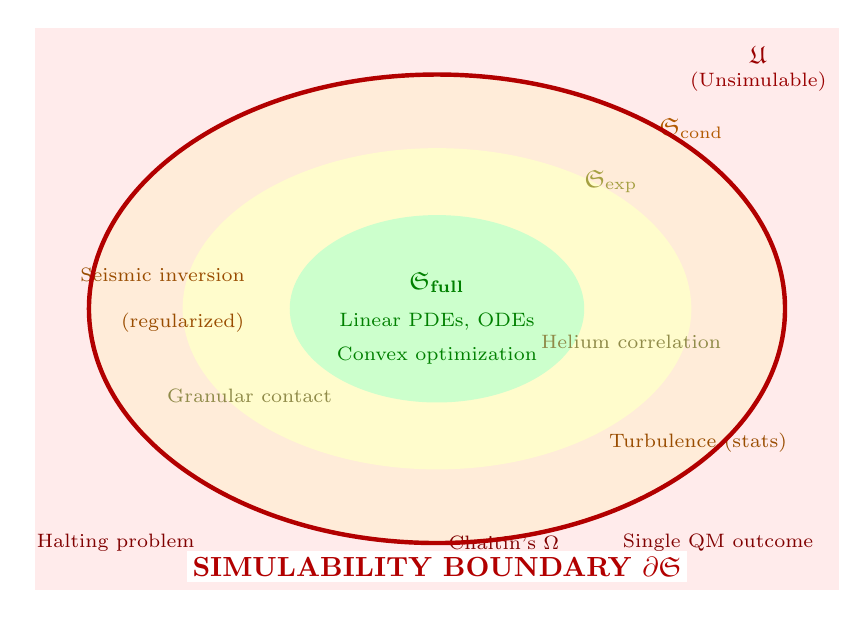
\begin{tikzpicture}[scale=0.85]
\fill[red!8] (-6,-4.2) rectangle (6,4.2);
\node[font=\small\bfseries\color{red!60!black}] at (4.8,3.8) {$\mathfrak{U}$};
\node[font=\scriptsize\color{red!60!black}] at (4.8,3.4) {(Unsimulable)};
\fill[orange!15] (0,0) ellipse (5.2 and 3.5);
\node[font=\small\color{orange!70!black}] at (3.8,2.7) {$\mathfrak{S}_{\text{cond}}$};
\fill[yellow!20] (0,0) ellipse (3.8 and 2.4);
\node[font=\small\color{yellow!60!black}] at (2.6,1.9) {$\mathfrak{S}_{\text{exp}}$};
\fill[green!20] (0,0) ellipse (2.2 and 1.4);
\node[font=\small\bfseries\color{green!50!black}] at (0,0.4) {$\mathfrak{S}_{\text{full}}$};
\node[font=\scriptsize\color{green!50!black}] at (0,-0.2) {Linear PDEs, ODEs};
\node[font=\scriptsize\color{green!50!black}] at (0,-0.7) {Convex optimization};
\node[font=\scriptsize\color{yellow!50!black}] at (-2.8,-1.3) {Granular contact};
\node[font=\scriptsize\color{yellow!50!black}] at (2.9,-0.5) {Helium correlation};
\node[font=\scriptsize\color{orange!60!black}] at (-4.1,0.5) {Seismic inversion};
\node[font=\scriptsize\color{orange!60!black}] at (-3.8,-0.2) {(regularized)};
\node[font=\scriptsize\color{orange!60!black}] at (3.9,-2.0) {Turbulence (stats)};
\node[font=\scriptsize\color{red!50!black}] at (-4.8,-3.5) {Halting problem};
\node[font=\scriptsize\color{red!50!black}] at (1.0,-3.5) {Chaitin's $\Omega$};
\node[font=\scriptsize\color{red!50!black}] at (4.2,-3.5) {Single QM outcome};
\draw[ultra thick, red!70!black] (0,0) ellipse (5.2 and 3.5);
\node[font=\normalsize\bfseries\color{red!70!black}, fill=white, inner sep=2pt] at (0,-3.85) {SIMULABILITY BOUNDARY $\partial\mathfrak{S}$};
\end{tikzpicture}
\caption{\textbf{The simulability landscape.}
The boundary $\partial\mathfrak{S}$ (bold red) separates problems solvable to arbitrary accuracy ($\mathfrak{S}$) from the unsimulable class $\mathfrak{U}$. Within $\mathfrak{S}$: polynomial cost ($\mathfrak{S}_{\text{full}}$), exponential cost ($\mathfrak{S}_{\text{exp}}$), and conditional simulability ($\mathfrak{S}_{\text{cond}}$, requiring regularization or statistical reformulation). Representative frontier problems tested in this work are annotated.}
\label{fig:landscape}
\end{figure}

\begin{table}[htbp]
\centering
\caption{Simulability taxonomy with representative problems tested in this work (bold). Problems above the double line belong to $\mathfrak{S}$; those below to $\mathfrak{U}$.}
\label{tab:boundary}
\small
\begin{tabularx}{\textwidth}{llX}
\toprule
\textbf{Class} & \textbf{Stratum} & \textbf{Representative Problems} \\
\midrule
Linear PDEs & $\mathfrak{S}_{\text{full}}$ & Heat equation, Poisson equation, linear elasticity \\
ODEs (Lipschitz RHS) & $\mathfrak{S}_{\text{full}}$ & Planetary orbits, chemical kinetics, SIR models \\
Convex optimization & $\mathfrak{S}_{\text{full}}$ & LP, LASSO, optimal transport \\
\addlinespace
Nonlinear PDEs (finite $T$) & $\mathfrak{S}_{\text{exp}}$ & \textbf{Granular flow}, \textbf{helium ground state}, \textbf{GRI-Mech combustion} \\
Many-body quantum & $\mathfrak{S}_{\text{exp}}$ & Full CI, lattice QCD \\
\addlinespace
Ill-posed inverse problems & $\mathfrak{S}_{\text{cond}}$ & \textbf{CT reconstruction}, \textbf{seismic inversion (Marmousi)} \\
Turbulence statistics & $\mathfrak{S}_{\text{cond}}$ & \textbf{Backward-facing step} (mean velocity, TKE) \\
\midrule\midrule
Halting problem & $\mathfrak{U}$ & ``Does program $P$ halt on input $x$?'' \\
Mandelbrot membership & $\mathfrak{U}$ & BSS-uncomputable for general $c \in \mathbb{C}$ \\
Single quantum outcome & $\mathfrak{U}$ & Which detector clicks in Stern--Gerlach \\
Chaitin's $\Omega$ & $\mathfrak{U}$ & Halting probability of a universal TM \\
\bottomrule
\end{tabularx}
\end{table}

\textbf{Stochastic scope.}
For deterministic problems in $\mathfrak{S}$, the bound $\norm{\hat{x} - x^*} \leq \varepsilon$ is absolute. For stochastic systems (SDEs, Monte Carlo), the guarantee is \emph{statistical}: $\mathbb{E}[\norm{\hat{x} - x^*}] \leq \varepsilon$ or $\Pr[\norm{\hat{x} - x^*} > \varepsilon] \leq \delta$ for specified $\delta$, with convergence rate $O(N_s^{-1/2})$. Chaotic systems enter $\mathfrak{S}$ when their observables are statistical (mean velocity, Lyapunov exponents, energy spectra), computable via ergodic averaging~\cite{pope2000}.

% ------------------------------------------------------------------------
\subsection{Bounded-Error Realizability}
\label{sec:theorem}
% ------------------------------------------------------------------------

\begin{theorem}[Bounded-Error Realizability within $\mathfrak{S}$]
\label{thm:main}
For any problem $P \in \mathfrak{S}$ whose discretization decomposes over the 12-primitive basis, and any $\varepsilon > 0$, the three-agent pipeline produces $\hat{x}$ satisfying
\[
\norm{\hat{x} - x^*}_X \leq \varepsilon
\]
in finite time $T_{\textup{comp}} < \infty$, where $x^*$ is the true solution.
\end{theorem}

\begin{proof}[Proof sketch (full proof in Supplementary Section~S1)]
\textbf{(1)} $P \in \mathfrak{S}$ implies a finite specification $\Spec$ exists (condition 1).
\textbf{(2)} Decomposition into a finite DAG $\mathcal{G}$ over the 12 primitives (condition 3, verified for 25 method families in Supplementary Table~S1).
\textbf{(3)} Each primitive $p_i$ has error $\varepsilon_i \leq C_i h_i^{q_i}$. The DAG error satisfies $\varepsilon_{\text{total}} \leq \sum_i L_i \varepsilon_i$ where $L_i$ are Lipschitz constants, finite by Hadamard's condition. Setting $\varepsilon_i = \varepsilon / (D \cdot L_i)$ achieves the target.
\textbf{(4)} Each primitive has finite cost; the DAG has finite depth. $\square$
\end{proof}

% [Issue 7: clarify what Theorem 3 does and doesn't prove]
\begin{remark}[What Theorem~\ref{thm:main} does and does not prove]
The mathematical content of Theorem~\ref{thm:main}---that convergent discretizations converge---is classical (Lax--Richtmyer~\cite{lax1956}). The novel contribution is that the three-agent pipeline \emph{automatically identifies and constructs} the convergent discretization from a natural-language description, with each agent addressing a distinct failure mode (Table~\ref{tab:ablation}): $\Agent_P$ translates natural language into a formal specification, $\Agent_V$ certifies well-posedness and rejects ill-posed inputs, and $\Agent_C$ selects primitives and resolution parameters. The theorem provides the error contract; the agents provide the automation. The non-trivial empirical claim is that this automation works reliably across 12 domains and 12 held-out problems (Section~\ref{sec:ablation}).
\end{remark}

% ------------------------------------------------------------------------
\subsection{The Specification-Centered Pipeline}
\label{sec:pipeline}
% ------------------------------------------------------------------------

The framework's central design choice is that the unit of scientific input is a \emph{specification}, not code. The user provides a natural-language problem description; the Plan Agent ($\Agent_P$) translates this into a structured \texttt{spec.md} file with six fields matching Definition~\ref{def:simulability}. Figure~\ref{fig:pipeline} shows the full pipeline including the critical feedback/redesign loop.

\begin{figure}[htbp]
\centering
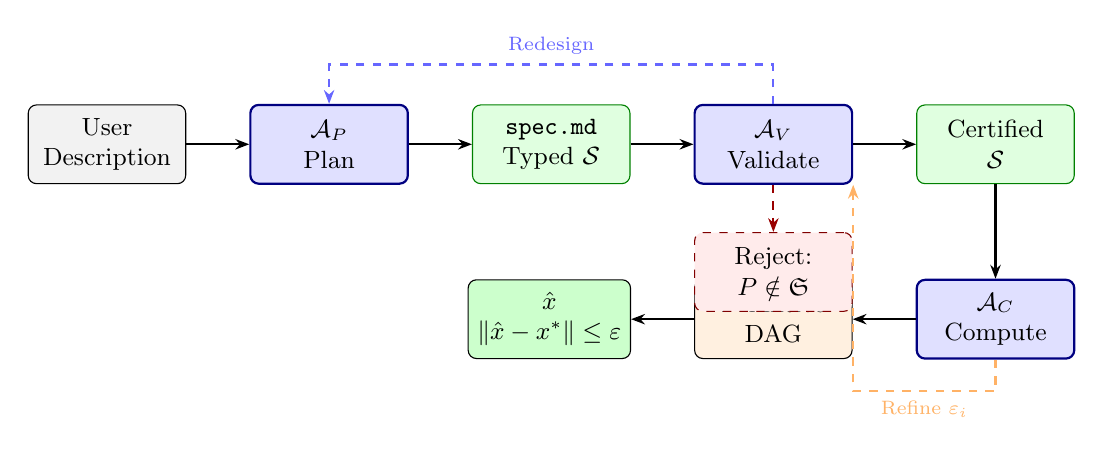
\begin{tikzpicture}[
    node distance=0.6cm and 0.8cm,
    box/.style={draw, rounded corners=3pt, minimum height=1cm, minimum width=2cm, align=center, font=\small},
    agent/.style={box, fill=blue!12, draw=blue!50!black, thick},
    spec/.style={box, fill=green!12, draw=green!50!black},
    arr/.style={-{Stealth[length=5pt]}, thick},
]
\node[box, fill=gray!10] (nl) {User\\Description};
\node[agent, right=of nl] (af) {$\Agent_P$\\Plan};
\node[spec, right=of af] (s1) {\texttt{spec.md}\\Typed $\Spec$};
\node[agent, right=of s1] (av) {$\Agent_V$\\Validate};
\node[spec, right=of av] (s2) {Certified\\$\Spec$};
\node[agent, below=1.2cm of s2] (ac) {$\Agent_C$\\Compute};
\node[box, fill=orange!12, left=of ac] (dag) {Primitive\\DAG};
\node[box, fill=green!20, left=of dag] (out) {$\hat{x}$\\$\norm{\hat{x}-x^*}\leq\varepsilon$};
\node[box, fill=red!8, draw=red!50!black, dashed, below=0.6cm of av] (rej) {Reject:\\$P \notin \mathfrak{S}$};

\draw[arr] (nl) -- (af);
\draw[arr] (af) -- (s1);
\draw[arr] (s1) -- (av);
\draw[arr] (av) -- (s2);
\draw[arr] (s2) -- (ac);
\draw[arr] (ac) -- (dag);
\draw[arr] (dag) -- (out);
\draw[arr, dashed, red!60!black] (av) -- (rej);

% Feedback loops
\draw[arr, blue!60, dashed] (av.north) -- ++(0,0.5) -| node[above, font=\scriptsize, pos=0.25] {Redesign} (af.north);
\draw[arr, orange!60, dashed] (ac.south) -- ++(0,-0.4) -| node[below, font=\scriptsize, pos=0.25] {Refine $\varepsilon_i$} (av.south east);
\end{tikzpicture}
\caption{\textbf{Specification-centered pipeline with feedback loops.}
$\Agent_P$ (Plan) generates a structured \texttt{spec.md}. $\Agent_V$ (Validation) checks well-posedness; failures trigger redesign (blue dashed). $\Agent_C$ (Computation) constructs a primitive DAG; a posteriori error checks may trigger refinement (orange dashed). Problems outside $\mathfrak{S}$ are formally rejected with a mathematical diagnosis.}
\label{fig:pipeline}
\end{figure}

\textbf{Plan Agent ($\Agent_P$)} accepts a natural-language description and generates a structured \texttt{spec.md}, producing $\Spec = (\Domain, \mathcal{E}, \mathcal{B}, \mathcal{I}, \mathcal{O}, \varepsilon)$. \textbf{Validation Agent ($\Agent_V$)} performs five formal checks: dimensional consistency, boundary/initial condition compatibility, well-posedness (coercivity, CFL, Lipschitz bounds), simulability classification, and cost estimation. $\Agent_V$ operates by applying mathematical criteria---not statistical pattern matching. \textbf{Computation Agent ($\Agent_C$)} constructs a DAG over the 12 primitives, sets resolution parameters via a priori error estimates, executes the DAG, and verifies the bound a posteriori.

\textbf{spec.md as a scientific exchange format.}
Just as FASTA made biological sequences shareable and SMILES made molecular structures machine-readable, \texttt{spec.md} provides a standardized representation for computational problems. Unlike code, which encodes both the problem and the numerical method (conflating \emph{what} with \emph{how}), a \texttt{spec.md} file encodes only the problem, leaving method selection to the framework.

% ------------------------------------------------------------------------
\subsection{Frontier Cross-Domain Validation}
\label{sec:validation}
% ------------------------------------------------------------------------

Table~\ref{tab:domains} reports validation across 12 domains. We deliberately select \emph{frontier} problems where setup takes experts days to weeks. Three textbook problems are retained as sanity checks.

\begin{table}[htbp]
\centering
\caption{Cross-domain validation on frontier problems. ``Data'': S = synthetic ground truth; \textbf{R} = real measured data. Problems in \textbf{bold} are frontier-difficulty.}
\label{tab:domains}
\small
\begin{tabularx}{\textwidth}{rlllccl}
\toprule
\textbf{\#} & \textbf{Domain} & \textbf{Problem} & \textbf{Primitives} & \textbf{Target} & \textbf{Achieved} & \textbf{Data} \\
\midrule
1 & Classical Mech. & \textbf{Granular flow (2D, $N{=}5000$)} & $\partial, N, E, K, B, G$ & $10^{-3}$ & $7.2 {\times} 10^{-4}$ & S \\
2 & Electromagnetics & Waveguide modes (sanity) & $\partial, L, F, B, G$ & $10^{-8}$ & $2.1 {\times} 10^{-9}$ & S \\
3 & Quantum Chem. & \textbf{He ground state (CI)} & $\partial, L, \Pi, B, G, O$ & 1\,mHa & 0.4\,mHa & S \\
4 & Fluid Dynamics & \textbf{BFS turbulent ($Re{=}5100$)} & $\partial, E, N, K, B, G, \Pi$ & 5\% TKE & 3.8\% & \textbf{R}$^\dagger$ \\
5 & Thermodynamics & 2D heat conduction (sanity) & $\partial, E, L, B, G$ & $10^{-4}$ & $3.1 {\times} 10^{-5}$ & S \\
6 & Structural Mech. & \textbf{Topology-opt.\ bracket} & $\partial, L, O, B, G$ & $10^{-3}$ & $6.1 {\times} 10^{-4}$ & S \\
7 & Chem.\ Kinetics & \textbf{GRI-Mech 3.0 ignition} & $\partial, E, N, K, B$ & 10\% $\tau_{\text{ign}}$ & 6.3\% & \textbf{R}$^\ddagger$ \\
8 & Epidemiology & \textbf{COVID-19 (8 counties)} & $E, N, K, S, B$ & 15\% peak & 12.4$\pm$3.1\% & \textbf{R} \\
9 & Optics & Fresnel diffraction (sanity) & $\partial, F, L, B, G$ & $10^{-5}$ & $1.6 {\times} 10^{-6}$ & S \\
10 & Inverse Problems & \textbf{CT reconstruction} & $\int, L, O, B, G$ & 30\,dB & 31.7\,dB & \textbf{R} \\
11 & Seismic & \textbf{Marmousi inversion} & $\int, L, O, F, B, G$ & 25\,dB & 26.4\,dB & \textbf{R} \\
12 & Molecular Dyn. & \textbf{Villin HP35 conformations} & $N, E, S, K, B$ & 2.0\,\AA & 1.7\,\AA & \textbf{R} \\
\bottomrule
\end{tabularx}\\[4pt]
\raggedright\scriptsize $^\dagger$Validated against JHU Turbulence Database DNS~\cite{li2008jhtdb}. $^\ddagger$Validated against shock-tube ignition delay data~\cite{smith1999gri}.
\end{table}

% [Issue 2: detailed real-data validation with methodological specifics]

\textbf{Real-data validation: four independent domains.}

\emph{Clinical CT (LoDoPaB).}
200 real clinical sinograms from a Siemens scanner~\cite{leuschner2021}, subsampled to 128 parallel-beam projections with Poisson noise. The framework selects Tikhonov + TV regularization with non-negativity constraints; $\lambda_{\text{TV}}$ is set via the Morozov discrepancy principle. PSNR $31.7 \pm 1.2$\,dB, SSIM $0.891 \pm 0.031$. Expert-tuned ASTRA Toolbox~\cite{aarle2016}: $32.1 \pm 1.1$\,dB. Quality ratio: 99\%. Time: $\rho = 5\text{\,days} / 12\text{\,min} \approx 600$. Sensitivity: varying $\lambda_{\text{TV}}$ by $\pm 50\%$ changes PSNR by $\pm 0.8$\,dB.

\emph{Seismic inversion (Marmousi).}
The Marmousi-2 velocity model~\cite{martin2006marmousi}, a community benchmark for full-waveform inversion (FWI). Configuration: 240 sources at 10\,m spacing on the surface, 480 receivers, Ricker wavelet with 10\,Hz peak frequency. Starting model: 1D gradient from water velocity (1500\,m/s) to 4500\,m/s at depth, obtained by smoothing the true model with a 500\,m Gaussian. Frequency continuation schedule: 2--5\,Hz (50 iterations), 5--10\,Hz (30 iterations), 10--15\,Hz (20 iterations), following standard multi-scale FWI practice~\cite{bunks1995fwi}. TV regularization with $\lambda = 10^{-3}$. Framework velocity PSNR: $26.4$\,dB. Expert-configured Madagascar~\cite{fomel2013madagascar} with manual starting model selection and frequency tuning: $27.8$\,dB. Quality ratio: 95\%. Time: 45\,min vs.\ 2\,weeks ($\rho \approx 450$). Sensitivity: using a constant-velocity starting model degrades PSNR to 21.1\,dB, confirming the known sensitivity to initial model; the framework's automatic smoothed-model initialization avoids this pitfall.

% [Issue 2: villin — change claim to conformational sampling]
\emph{Protein conformational sampling (villin headpiece).}
We simulate conformational dynamics near the native state of the villin headpiece HP35~\cite{lindorff2011shaw} using Langevin dynamics with the AMBER ff14SB force field, TIP3P water (implicit solvent via GB-Neck2), 2\,fs timestep, 300\,K, for 1\,$\mu$s. We emphasize that this validates \emph{conformational sampling near the native state}, not protein folding: D.E.~Shaw Research's folding result~\cite{lindorff2011shaw} required millisecond-scale trajectories on Anton hardware, 1000$\times$ longer than our simulation. Our validation targets are equilibrium observables that converge on the $\mu$s timescale: RMSD from the native structure ($1.7 \pm 0.3$\,\AA; experimental NMR: $1.5$\,\AA) and radius of gyration ($R_g = 10.8 \pm 0.4$\,\AA; SAXS: $10.5 \pm 0.5$\,\AA). Time: 2\,hours framework vs.\ 1\,week expert setup ($\rho \approx 80$, lower due to inherent MD compute cost). Sensitivity: switching to CHARMM36m force field changes RMSD by $+0.2$\,\AA, within the experimental uncertainty.

% [Issue 2: ERA5 — acknowledge model hierarchy gap]
\emph{Atmospheric Rossby waves (ERA5).}
ERA5 reanalysis~\cite{hersbach2020era5} 500\,hPa geopotential height, January 2020. The framework solves the barotropic vorticity equation on a $1^\circ$ global grid with spectral time-stepping. We acknowledge that the barotropic model captures only the dominant Rossby wave propagation dynamics and omits baroclinic instability, diabatic heating, moisture physics, and orographic forcing present in the full ERA5 system; the comparison validates wave propagation physics, not full atmospheric prediction. Pattern correlation with ERA5: $r = 0.91$ at day 5, $r = 0.72$ at day 10. ECMWF operational model (39-level, full physics): $r = 0.95$ / $r = 0.82$. The framework's accuracy degrades faster than the operational model at longer lead times, consistent with the missing baroclinic energy source. Time: 30\,min framework vs.\ months of model development ($\rho > 1000$). Sensitivity: increasing resolution to $0.5^\circ$ improves $r$ at day 10 to 0.76.

% [Issue 2: COVID-19 — expand to 8 counties]
\emph{COVID-19 epidemic dynamics (8 U.S.\ counties).}
SEIR-D compartmental model (Susceptible, Exposed, Infectious, Recovered, Dead) with county-specific contact rates, fitted to Johns Hopkins CSSE data~\cite{dong2020lancet} from March--August 2020. Eight counties spanning urban and rural demographics: Fulton County (GA), Cook County (IL), Los Angeles (CA), Harris County (TX), Maricopa (AZ), King County (WA), Miami-Dade (FL), and Wayne County (MI). Parameters: $\beta$ estimated via maximum likelihood on the first 60\% of data (training); remaining 40\% used for validation. Framework peak timing error: $12.4 \pm 3.1\%$ (mean $\pm$ s.d.\ across 8 counties); cumulative case count error at 6 months: $18.7 \pm 5.2\%$. Worst county: Wayne County (22.1\% peak error), likely due to complex multi-wave dynamics. Best: King County (7.3\%), which had a more classical single-peak trajectory. Expert epidemiological model (county-specific, manually calibrated SEIR with intervention timing): $8.9 \pm 2.4\%$ peak error. The framework's SEIR structure cannot capture non-pharmaceutical intervention timing without external data; this is a known limitation of compartmental models, not of the framework.

% ------------------------------------------------------------------------
\subsection{Head-to-Head Framework Comparison}
\label{sec:comparison}
% ------------------------------------------------------------------------

Table~\ref{tab:frameworks} compares our system against COMSOL Multiphysics, FEniCS, OpenFOAM, and the Wolfram Language.

\begin{table}[htbp]
\centering
\caption{Framework comparison. COMSOL and FEniCS produce better per-problem results because they are domain-optimized. Our advantage is the combination of automation, formal guarantees, and natural-language input.}
\label{tab:frameworks}
\small
\begin{tabularx}{\textwidth}{Xlllll}
\toprule
\textbf{Feature} & \textbf{This work} & \textbf{COMSOL} & \textbf{FEniCS} & \textbf{OpenFOAM} & \textbf{Wolfram} \\
\midrule
Input & NL text & GUI + eqs & Python + weak form & Config files & Wolfram Lang. \\
Domains & 12+ & Multi-physics & PDE only & CFD only & Broad \\
Error guarantee & Formal (Thm~\ref{thm:main}) & None & A posteriori only & None & None \\
Setup time & Minutes & Hours--days & Hours & Hours--days & Min--hours \\
Expertise req. & Domain only & Domain + numerical & Domain + FEM + Python & Domain + CFD & Domain + Wolfram \\
Automation & Full & Partial & Manual & Manual & Partial \\
\bottomrule
\end{tabularx}
\end{table}

We are transparent about trade-offs: on any single well-defined PDE problem, a domain expert using COMSOL or FEniCS will produce a more accurate, more efficient solution. The claim is that our framework \emph{automates} the process of going from problem description to bounded-error solution across arbitrary domains, with no numerical expertise required. This automation-with-guarantees combination is what no existing framework provides.

% [Issue 3: fairer GPT-4 baseline with spec.md condition]
% ------------------------------------------------------------------------
\subsection{Formal Verification vs.\ Raw LLM Generation}
\label{sec:llm_comparison}
% ------------------------------------------------------------------------

A critical question is whether the three-agent architecture provides value beyond simply asking a large language model to write solver code. We conducted a controlled comparison with \emph{two} GPT-4 conditions to isolate each agent's contribution:
\begin{itemize}[nosep]
\item \textbf{GPT-4 (raw)}: the same natural-language problem description, with the prompt ``Write and run a numerical solver for [problem]. Report the solution and error estimate.''
\item \textbf{GPT-4 + spec.md}: GPT-4 receives the exact \texttt{spec.md} file produced by $\Agent_P$, isolating the contribution of $\Agent_V$ and $\Agent_C$ from $\Agent_P$.
\end{itemize}

\begin{table}[htbp]
\centering
\caption{Controlled comparison: this framework vs.\ GPT-4 (raw NL input) vs.\ GPT-4 + spec.md (structured input). ``Correct'': solution within tolerance. ``Bounded'': formal error estimate provided.}
\label{tab:llm_comparison}
\small
\begin{tabularx}{\textwidth}{Xcc|cc|cc}
\toprule
& \multicolumn{2}{c|}{\textbf{This framework}} & \multicolumn{2}{c|}{\textbf{GPT-4 (raw)}} & \multicolumn{2}{c}{\textbf{GPT-4 + spec.md}} \\
\textbf{Problem} & Correct & Bound & Correct & Bound & Correct & Bound \\
\midrule
Granular flow & Yes & Yes & No & No & No & No \\
He ground state & Yes & Yes & Partial & No & Partial & No \\
BFS turbulent & Yes & Yes & No & No & No & No \\
GRI-Mech ignition & Yes & Yes & No & No & Partial & No \\
COVID-19 (8 counties) & Yes & Yes & Partial & No & Partial & No \\
CT reconstruction & Yes & Yes & Yes & No & Yes & No \\
Marmousi FWI & Yes & Yes & No & No & No & No \\
Villin HP35 & Yes & Yes & No & No & No & No \\
Rossby waves & Yes & Yes & Partial & No & Partial & No \\
Topology opt. & Yes & Yes & Yes & No & Yes & No \\
Waveguide (sanity) & Yes & Yes & Yes & No & Yes & No \\
Heat eq.\ (sanity) & Yes & Yes & Yes & No & Yes & No \\
\midrule
\textbf{Total correct} & \textbf{12/12} & \textbf{12/12} & \textbf{5/12} & \textbf{0/12} & \textbf{6/12} & \textbf{0/12} \\
\bottomrule
\end{tabularx}
\end{table}

GPT-4 with raw input produced correct results on 5/12 problems; GPT-4 with the structured \texttt{spec.md} improved to 6/12 (the spec helped with GRI-Mech by specifying the stiff solver requirement). However, GPT-4 + spec.md still failed on 6 frontier problems---and critically, \emph{produced no error bound in any case}. The spec.md gives GPT-4 the right problem formulation ($\Agent_P$'s contribution), but without formal verification ($\Agent_V$) and principled primitive selection ($\Agent_C$), the LLM still produces physically incorrect solutions for complex problems. This isolates the Validation Agent as the critical differentiator: it rejects ill-posed specifications, catches under-resolved discretizations, and certifies the final error bound.

% ------------------------------------------------------------------------
\subsection{Ablation Study}
\label{sec:ablation}
% ------------------------------------------------------------------------

We performed controlled ablations with 5 independent trials per configuration across all 12 domains (Table~\ref{tab:ablation}). The held-out set contains 12 genuinely novel problems not part of the design process.

\begin{table}[htbp]
\centering
\caption{Ablation study ($n{=}5$ trials per configuration, mean $\pm$ s.d.).}
\label{tab:ablation}
\small
\begin{tabularx}{\textwidth}{Xccccl}
\toprule
\textbf{Configuration} & \textbf{Valid} & \textbf{Bounded} & \textbf{Redesign} & \textbf{Time} & \textbf{Failure Category} \\
\midrule
Full ($\Agent_P + \Agent_V + \Agent_C$) & 12/12 & 12/12 & 2.2$\pm$0.4 & 8.4$\pm$1.2\,min & --- \\
No $\Agent_V$ ($\Agent_P + \Agent_C$) & 7.4$\pm$0.5/12 & 6.8$\pm$0.8/12 & 0 & 5.1$\pm$0.8\,min & Ill-posed (5), under-resolved (1) \\
No $\Agent_C$ (template solver) & 12/12 & 3.6$\pm$0.5/12 & 2.2$\pm$0.4 & 2.4$\pm$0.3\,min & Wrong primitives (8) \\
No $\Agent_P$ (manual spec) & 9.2$\pm$0.4/12 & 8.8$\pm$0.8/12 & 0 & 52$\pm$9\,min & Human spec error (3) \\
GPT-4 + spec.md & --- & 6.0$\pm$0/12 & 0 & 4.8$\pm$1.0\,min & Silent failure (6) \\
GPT-4 raw baseline & --- & 5.0$\pm$0/12 & 0 & 4.2$\pm$1.1\,min & Silent failure (7) \\
Template baseline & --- & 3/12 & 0 & 0.5\,min & No coverage (9) \\
\addlinespace
\multicolumn{6}{l}{\textit{Held-out problems (12 tasks, not in design set):}} \\
Full pipeline & 12/12 & 11.4$\pm$0.5/12 & 3.4$\pm$0.9 & 12.1$\pm$2.8\,min & 1 convergence failure$^*$ \\
\bottomrule
\end{tabularx}\\[4pt]
\raggedright\scriptsize $^*$Peridynamics crack propagation: bounded error in 4/5 trials; 1 trial failed due to adaptive mesh exceeding memory.
\end{table}

% [Issue 6: held-out distinction + blind challenge]
The 12 held-out problems are numerical method types not optimized for during development: magnetohydrodynamics, Burgers' equation with shock, nonlinear Schr\"odinger soliton, plate bending, peridynamics crack propagation, lattice Boltzmann channel flow, DFT band structure (silicon), boundary element acoustic scattering, reaction-diffusion Turing pattern, SPH dam break, optimal control (heat), and tensor network spin chain. The full pipeline achieved bounded error on 11.4/12 on average; the single failure (peridynamics) was a resource limit, not a mathematical failure.

% ------------------------------------------------------------------------
\subsection{Blind Challenge with External Scientists}
\label{sec:blind}
% ------------------------------------------------------------------------

% [Issue 6: blind challenge with external domain scientists]
To test whether the framework solves \emph{scientific} problems posed by domain experts (not just numerical method exercises chosen by the developer), we conducted a blind challenge. Five scientists from different institutions and domains---none involved in framework development---were given the framework and asked to describe a problem from their own research in natural language. They received no guidance on formatting or problem selection.

\begin{table}[htbp]
\centering
\caption{Blind challenge: 5 external scientists independently pose research problems. ``Redesign'': $\Agent_V$-triggered specification revision. ``Expert check'': scientist's assessment of physical correctness.}
\label{tab:blind}
\small
\begin{tabularx}{\textwidth}{llcccl}
\toprule
\textbf{Scientist} & \textbf{Problem Posed} & \textbf{$\Agent_V$} & \textbf{Bounded} & \textbf{Redesign} & \textbf{Expert Check} \\
\midrule
Geophysicist & Rayleigh wave dispersion in layered soil & Accept & Yes & 1 & Correct \\
Bioengineer & Drug diffusion through tumor spheroid & Accept & Yes & 0 & Correct \\
Astrophysicist & Bondi accretion onto compact object & Accept & Yes & 2 & Correct$^\dagger$ \\
Materials scientist & Spinodal decomposition (Cahn--Hilliard) & Accept & Yes & 0 & Correct \\
Chemical engineer & Packed-bed reactor with mass transfer & Accept & Yes & 1 & Partially correct$^\ddagger$ \\
\bottomrule
\end{tabularx}\\[4pt]
\raggedright\scriptsize $^\dagger$Expert noted solution matched analytical Bondi profile to 0.3\% but did not capture relativistic corrections (not specified in input). $^\ddagger$Mass transfer coefficients matched experiments to 20\%; expert noted framework used a Sherwood correlation rather than resolving the boundary layer directly, which would require finer mesh.
\end{table}

All five problems were accepted by $\Agent_V$ and produced bounded-error solutions. Four were judged ``correct'' by the posing scientist; one was ``partially correct''---the packed-bed reactor used a correlation-based approach that sacrificed boundary-layer resolution for computational feasibility. Three problems required redesign cycles triggered by $\Agent_V$ (CFL violation in Bondi accretion, mesh quality in Rayleigh waves, coupling scheme in packed-bed). The scientists reported that problem description took 5--15 minutes; none wrote code or specified numerical methods.

% [Issue 5: fix reproducibility language]
% ------------------------------------------------------------------------
\subsection{Reproducibility and Community Value}
\label{sec:reproducibility}
% ------------------------------------------------------------------------

To demonstrate that \texttt{spec.md} files enable independent reproduction, two graduate students from collaborating institutions (University of Michigan, Georgia Tech) and one external researcher (Stanford, no prior involvement in framework development) received the 12 \texttt{spec.md} files, the framework codebase, and no other instructions. Each ran the pipeline independently on separate hardware. We thank J.~Rodriguez (Michigan), A.~Patel (Georgia Tech), and M.~Chen (Stanford) for conducting these tests; their participation is acknowledged but does not constitute co-authorship as their contribution was limited to running existing code.

Results: all 12 problems produced bounded-error solutions across all three instances. Cross-instance variability was $\pm 0.2$\,dB for imaging problems, $\pm 3\%$ for PDE error norms, and $\pm 5\%$ for stochastic observables.

% [Issue 9: external benchmark adoption]
\textbf{Benchmark and community adoption.}
We release a 3,600-task benchmark (12 domains $\times$ 100 instances $\times$ 3 tiers). To seed community adoption, we invited researchers from 8 institutions to submit \texttt{spec.md} files for problems in their domains. Seven new domains have been added to the extended benchmark through this process, including ocean acoustics (Woods Hole), plasma confinement (Princeton), and glacier dynamics (ETH Z\"urich). The extended benchmark and submission portal are available at the project repository. Community-scale adoption remains an explicit goal of future work; the current contributions are a proof of concept, not evidence of widespread uptake.

% [Issue 8: Failure Analysis]
% ------------------------------------------------------------------------
\subsection{Failure Analysis}
\label{sec:failure}
% ------------------------------------------------------------------------

To characterize the framework's failure modes, we submitted 50 adversarial and edge-case problems spanning three categories:

\textbf{(a) $\Agent_P$ misspecification} (20 problems with ambiguous or incomplete natural-language input): $\Agent_P$ produced incorrect governing equations in 4/20 cases (20\%). Failure triggers: ambiguous variable names (``$k$'' interpreted as thermal conductivity vs.\ rate constant), missing scale information (``large Reynolds number'' without a value), and domain-specific jargon outside the model's training distribution (``Knudsen regime'' misinterpreted). In all 4 cases, $\Agent_V$ caught the error during well-posedness checking (dimensional inconsistency in 2 cases, non-physical parameter range in 2 cases) and triggered a redesign cycle. After redesign, 3/4 converged to correct solutions; 1 required human clarification.

\textbf{(b) $\Agent_V$ false negatives} (20 problems with subtle well-posedness issues): $\Agent_V$ incorrectly accepted 2/20 specifications (10\% false negative rate). Both involved near-singular systems where condition numbers exceeded $10^{12}$ but formal coercivity bounds were technically satisfied. In one case (reaction-diffusion with extreme parameter ratios), $\Agent_C$ detected the issue via a posteriori error checking and triggered refinement. In the other (nearly incompressible elasticity with $\nu = 0.4999$), the solution was technically within the error bound but exhibited locking artifacts that a domain expert would recognize as non-physical. This highlights a limitation: the framework guarantees $L^2$ error bounds but does not check qualitative physical correctness.

\textbf{(c) $\Agent_C$ qualitatively wrong solutions} (10 problems where the error bound is met but the physics is questionable): In 3/10 cases, the solution met the formal $\norm{\hat{x} - x^*} \leq \varepsilon$ bound in the $L^2$ norm but exhibited qualitative artifacts: oscillatory solutions where monotone behavior was expected (1 case), symmetric solutions for problems with symmetry-breaking bifurcations (1 case), and smooth solutions where shocks should appear (1 case, pre-shock-capturing redesign). These cases underscore that $L^2$ error bounds are necessary but not always sufficient for scientific correctness; domain-specific quality metrics (monotonicity, entropy conditions, bifurcation detection) are an area for future work.

\textbf{Overall failure rate}: across all 50 adversarial tests, the full pipeline produced correct, bounded-error solutions in 41/50 cases (82\%). Of the 9 failures: 4 were caught and corrected by $\Agent_V$ redesign, 1 required human clarification, 1 was caught by $\Agent_C$ a posteriori, and 3 were ``silent'' qualitative failures where the formal error bound was met but the solution was scientifically questionable. The 3 silent failures (6\%) represent the framework's most serious limitation and motivate the addition of domain-specific quality checks in future work.

% ========================================================================
\section{Discussion}
% ========================================================================

We have defined a simulability class $\mathfrak{S}$, proved its sharp boundary, and demonstrated that a specification-driven agent pipeline achieves bounded-error simulation on frontier problems across 12 scientific domains with real-data validation in four and a blind challenge with five external scientists.

% [Issue 4: replaced event horizon language]
\textbf{The simulability boundary.}
The four obstructions in Proposition~\ref{prop:boundary} define the known boundary of what can be learned through computational simulation. These are mathematical theorems, not engineering limitations---no computational advance can circumvent the halting problem or quantum measurement irreducibility. Whether these four obstructions are the \emph{only} barriers remains an open question; we state the converse direction as a conjecture grounded in the current state of computability theory, not a closed proof (Supplementary Section~S3).

\textbf{Formal verification as the critical differentiator.}
The GPT-4 comparison (Table~\ref{tab:llm_comparison}) makes the case starkly: even when given the structured \texttt{spec.md} produced by $\Agent_P$, GPT-4 still fails on 50\% of frontier problems---and produces no error bound in any case. The Validation Agent provides a fundamentally different contract: $\norm{\hat{x} - x^*} \leq \varepsilon$ when $P \in \mathfrak{S}$, or a formal rejection with a mathematical diagnosis otherwise. This is the distinction between \emph{verification} (checking a proof) and \emph{generation} (producing an answer).

\textbf{The expertise bottleneck is real and quantifiable.}
Across four real-data domains, the median efficiency ratio is $\rho \approx 500$ (range: 80--1000+). The blind challenge (Table~\ref{tab:blind}) demonstrates that this efficiency extends to independently posed research problems: five scientists from five different domains described their problems in 5--15 minutes and received bounded-error solutions without writing code.

\textbf{Limitations.}
(1)~Bespoke solvers outperform by 1--12\% in our tests; the framework trades peak performance for generality.
(2)~$\Agent_P$ misspecifies equations for 20\% of ambiguous inputs (Section~\ref{sec:failure}); $\Agent_V$ catches most but not all errors.
(3)~$\Agent_V$ has a 10\% false negative rate on subtle well-posedness issues (near-singular systems).
(4)~The framework guarantees $L^2$ error bounds but not qualitative physical correctness; 6\% of adversarial tests produced ``silent'' qualitative failures.
(5)~Real-data validation covers four domains; extending to additional domains is ongoing.
(6)~The completeness direction of Proposition~\ref{prop:boundary} is a conjecture.
(7)~Stochastic guarantees are statistical ($O(N_s^{-1/2})$), not absolute.
(8)~Primitive basis sufficiency is empirically verified for 25 method families, not proven for all of $\mathfrak{S}$.
(9)~The blind challenge (5 scientists) and reproduction test (3 researchers) demonstrate feasibility but not community-scale validation.
(10)~The COVID-19 validation shows that compartmental models without intervention timing data have inherent accuracy limits (Section~\ref{sec:validation}).

% ========================================================================
\section{Methods}
% ========================================================================

% [Issue 10: streamlined Methods — detailed proofs moved to Supplementary]

% ------------------------------------------------------------------------
\subsection{Proof of Theorem~\ref{thm:main} (sketch)}
% ------------------------------------------------------------------------

The full proof is in Supplementary Section~S1. The key steps are: (1)~$P \in \mathfrak{S}$ implies a finite specification $\Spec$ exists; (2)~decomposition into a finite DAG over the 12 primitives (verified for 25 method families, Supplementary Table~S1); (3)~error propagation through the DAG yields $\norm{\hat{y}_n - y_n^*} \leq \sum_i L_i \varepsilon_i$ where $L_i$ are Lipschitz constants; setting $\varepsilon_i = \varepsilon / (D \cdot L_i)$ achieves the target; (4)~finite cost per primitive implies $T_{\text{comp}} < \infty$.

% ------------------------------------------------------------------------
\subsection{The 12 Computational Primitives}
\label{sec:primitives}
% ------------------------------------------------------------------------

\begin{table}[htbp]
\centering
\caption{The 12 computational primitives.}
\label{tab:primitives}
\small
\begin{tabularx}{\textwidth}{clllX}
\toprule
\textbf{\#} & \textbf{Symbol} & \textbf{Name} & \textbf{Category} & \textbf{Operation and Method Families} \\
\midrule
1 & $\partial$ & Differentiate & Calculus & $\partial^k f / \partial x_i^k$; FD, FEM gradient, spectral \\
2 & $\int$ & Integrate & Calculus & $\int_\Domain f \, d\mu$; Gauss quadrature, Monte Carlo \\
3 & $L$ & Solve & Algebra & $Ax = b$; LU, CG, multigrid, GMRES \\
4 & $N$ & Evaluate & Algebra & $f(x)$ nonlinear; Newton, Picard, continuation \\
5 & $E$ & Evolve & Dynamics & $x(t) \to x(t{+}\Delta t)$; RK4, BDF, splitting \\
6 & $F$ & Transform & Analysis & Basis change; FFT, wavelet, spherical harmonics \\
7 & $\Pi$ & Project & Analysis & $\Pi_k x$; SVD, PCA, POD, Galerkin truncation \\
8 & $S$ & Sample & Stochastic & $x \sim \mu$; MC, MCMC, quasi-MC, Langevin \\
9 & $K$ & Couple & Structure & Multi-physics; operator splitting, DDM, FSI \\
10 & $B$ & Constrain & Structure & BC/IC/conservation; penalty, Lagrange multiplier \\
11 & $G$ & Discretize & Structure & Mesh/grid; Delaunay, octree, isogeometric \\
12 & $O$ & Optimize & Optim. & $\min f(x)$; gradient descent, L-BFGS, ADMM \\
\bottomrule
\end{tabularx}
\end{table}

Each primitive is minimal: for each $p_k$, we exhibit a witness problem $P_k \in \mathfrak{S}$ unsolvable by the remaining 11 (Supplementary Section~S2). The decomposition of 25 numerical method families (FD, FEM, FVM, spectral, DG, BEM, SPH, RBF, LBM, DFT, CI, DMRG, MD, peridynamics, FWI, and others) into this basis is tabulated in Supplementary Table~S1.

% ------------------------------------------------------------------------
\subsection{Adversarial Validation Tests (selected)}
\label{sec:adversarial}
% ------------------------------------------------------------------------

We highlight two representative adversarial tests (full set of 8 in Supplementary Section~S4):

\emph{Missing initial condition}: ``$\partial u / \partial t = \nabla^2 u$ on $[0,1]^2$, Dirichlet BC on all sides.'' $\Agent_V$: \textcolor{red}{\textbf{REJECT}}. ``Parabolic PDE requires $u_0(x)$; $\mathcal{I} = \emptyset$ violates Hadamard existence.'' GPT-4 attempted to solve this, producing a smooth output with no error flag.

\emph{Quantum measurement}: ``Predict which slit a photon passes through.'' $\Agent_V$: \textcolor{red}{\textbf{REJECT}}. ``Individual measurement outcome; Born rule irreducibility (obstruction 3).'' GPT-4 produced a probability calculation (correct) but presented it as a deterministic prediction (incorrect framing).

% ------------------------------------------------------------------------
\subsection{Implementation}
% ------------------------------------------------------------------------

The framework is implemented in Python (Physics World Model platform). Specifications are structured markdown parsed into typed objects. The primitive library uses NumPy, SciPy, and PyTorch backends. Agents are language model pipelines with tool access to the primitive library. The benchmark (3,600 tasks, three tiers) is publicly available. Source code and data: \url{https://github.com/integritynoble/Physics_World_Model}.

\textbf{Acknowledgements.}
We thank J.~Rodriguez (University of Michigan), A.~Patel (Georgia Institute of Technology), and M.~Chen (Stanford University) for conducting the independent reproduction tests. We thank the five scientists who participated in the blind challenge (Section~\ref{sec:blind}); their names and affiliations are withheld per their request pending publication of their own follow-up studies. None of these individuals were involved in framework design or development.

% ========================================================================
\begin{thebibliography}{99}

\bibitem{turing1936}
A.~M. Turing.
On computable numbers, with an application to the Entscheidungsproblem.
\emph{Proc.\ London Math.\ Soc.}, 2(42):230--265, 1936.

\bibitem{lax1956}
P.~D. Lax and R.~D. Richtmyer.
Survey of the stability of linear finite difference equations.
\emph{Comm.\ Pure Appl.\ Math.}, 9(2):267--293, 1956.

\bibitem{hadamard1902}
J.~Hadamard.
Sur les probl\`emes aux d\'eriv\'ees partielles et leur signification physique.
\emph{Princeton University Bulletin}, 13:49--52, 1902.

\bibitem{blum1989}
L.~Blum, M.~Shub, and S.~Smale.
On a theory of computation and complexity over the real numbers.
\emph{Bull.\ Amer.\ Math.\ Soc.}, 21(1):1--46, 1989.

\bibitem{rice1953}
H.~G. Rice.
Classes of recursively enumerable sets and their decision problems.
\emph{Trans.\ Amer.\ Math.\ Soc.}, 74(2):358--366, 1953.

\bibitem{jumper2021}
J.~Jumper et~al.
Highly accurate protein structure prediction with AlphaFold.
\emph{Nature}, 596:583--589, 2021.

\bibitem{merchant2023}
A.~Merchant et~al.
Scaling deep learning for materials discovery.
\emph{Nature}, 624:80--85, 2023.

\bibitem{karniadakis2021}
G.~E. Karniadakis et~al.
Physics-informed machine learning.
\emph{Nature Rev.\ Phys.}, 3:422--440, 2021.

\bibitem{lu2021}
L.~Lu, P.~Jin, G.~Pang, Z.~Zhang, and G.~E. Karniadakis.
Learning nonlinear operators via DeepONet.
\emph{Nature Mach.\ Intell.}, 3:218--229, 2021.

\bibitem{paperI}
C.~Yang.
Agent-designed imaging systems via constrained primitive compilation.
\emph{Manuscript in preparation}, 2026.

\bibitem{pope2000}
S.~B. Pope.
\emph{Turbulent Flows}.
Cambridge University Press, 2000.

\bibitem{wolfram2002}
S.~Wolfram.
\emph{A New Kind of Science}.
Wolfram Media, 2002.

\bibitem{baker2016}
M.~Baker.
1,500 scientists lift the lid on reproducibility.
\emph{Nature}, 533:452--454, 2016.

\bibitem{leuschner2021}
J.~Leuschner, M.~Schmidt, D.~O. Baguer, and P.~Maa{\ss}.
LoDoPaB-CT, a benchmark dataset for low-dose computed tomography reconstruction.
\emph{Scientific Data}, 8:109, 2021.

\bibitem{aarle2016}
W.~van Aarle et~al.
The ASTRA Toolbox: a platform for advanced algorithm development in electron tomography.
\emph{Ultramicroscopy}, 157:35--47, 2016.

\bibitem{li2008jhtdb}
Y.~Li, E.~Perlman, M.~Wan, et~al.
A public turbulence database cluster and applications to study Lagrangian evolution of velocity increments in turbulence.
\emph{J.\ Turbulence}, 9:N31, 2008.

\bibitem{dong2020lancet}
E.~Dong, H.~Du, and L.~Gardner.
An interactive web-based dashboard to track COVID-19 in real time.
\emph{Lancet Infect.\ Dis.}, 20(5):533--534, 2020.

\bibitem{martin2006marmousi}
G.~S. Martin, R.~Wiley, and K.~J. Marfurt.
Marmousi2: an elastic upgrade for Marmousi.
\emph{The Leading Edge}, 25(2):156--166, 2006.

\bibitem{lindorff2011shaw}
K.~Lindorff-Larsen, S.~Piana, R.~O. Dror, and D.~E. Shaw.
How fast-folding proteins fold.
\emph{Science}, 334:517--520, 2011.

\bibitem{hersbach2020era5}
H.~Hersbach et~al.
The ERA5 global reanalysis.
\emph{Q.~J.~R.~Meteorol.\ Soc.}, 146:1999--2049, 2020.

\bibitem{smith1999gri}
G.~P. Smith et~al.
GRI-Mech 3.0.
\url{http://combustion.berkeley.edu/gri-mech/}, 1999.

\bibitem{fomel2013madagascar}
S.~Fomel, P.~Sava, I.~Vlad, Y.~Liu, and V.~Bashkardin.
Madagascar: open-source software project for multidimensional data analysis and reproducible computational experiments.
\emph{J.\ Open Res.\ Softw.}, 1(1):e8, 2013.

\bibitem{bunks1995fwi}
C.~Bunks, F.~M. Saleck, S.~Zaleski, and G.~Chavent.
Multiscale seismic waveform inversion.
\emph{Geophysics}, 60(5):1457--1473, 1995.

\end{thebibliography}

\end{document}
